\documentclass[11pt,letterpaper,article,oneside]{memoir}
\usepackage[utf8]{inputenc}
\usepackage[T1]{fontenc}
\usepackage{microtype}
\usepackage[dvips]{graphicx}
\usepackage{xcolor}
\usepackage{times}

\usepackage{booktabs}

\usepackage{enumitem}
\setlist[description]{style=nextline}
\setlist[itemize]{nosep}

\usepackage[
breaklinks=true,colorlinks=true,
linkcolor=blue,urlcolor=blue,citecolor=blue,% PDF VIEW
%linkcolor=black,urlcolor=black,citecolor=black,% PRINT
bookmarks=true,bookmarksopenlevel=2]{hyperref}

\usepackage{geometry}
% PDF VIEW
% \geometry{total={210mm,297mm},
% left=25mm,right=25mm,%
% bindingoffset=0mm, top=25mm,bottom=25mm}
% PRINT
\geometry{total={210mm,297mm},
left=20mm,right=20mm,
bindingoffset=10mm, top=25mm,bottom=25mm}

\OnehalfSpacing

%%% STYLE OF SECTIONS, SUBSECTIONS, AND SUBSUBSECTIONS
\setsecheadstyle{\large\bfseries\raggedright}
\setsubsecheadstyle{\bfseries\raggedright}


%%% STYLE OF PAGES NUMBERING
\pagestyle{plain}
\makepagestyle{plain}
\makeevenfoot{plain}{\thepage}{}{}
\makeoddfoot{plain}{}{}{\thepage}
\makeevenhead{plain}{}{}{}
\makeoddhead{plain}{}{}{}

\maxsecnumdepth{section}
\maxtocdepth{section}



\newcommand{\name}{IMU-Capture}
\newcommand{\programVersion}{0.1}
\newcommand{\manualVersion}{0.1}
\newcommand{\email}{eric.tytell@tufts.edu}

\newcommand{\csv}{\texttt{.csv}}
\newcommand{\hdf}{\texttt{.hdf5}}


\renewcommand{\arraystretch}{1.2}

\setlength{\parindent}{0em}
\nonzeroparskip





\begin{document}

\thispagestyle{empty}

{%%%
\centering
\Large

\vspace*{\fill}

{\huge
\name{} \programVersion{}
}

{\LARGE
User manual
}

\today

\vspace*{\fill}

}

\cleardoublepage

\tableofcontents*

\clearpage



%%%%%%%%%%%%%%%%%%%%%%%%%%%%%%%%%%%%%%%%%%%%%%
%                 LICENSE                    %
%%%%%%%%%%%%%%%%%%%%%%%%%%%%%%%%%%%%%%%%%%%%%%

\chapter{Copyright and License}

\name{}: a tool for collecting IMU measurements.
Copyright (C) 2017 David Buckingham, Eric Tytell, Vishesh Vikas

This program is free software: you can redistribute it and/or modify
it under the terms of the GNU General Public License as published by
the Free Software Foundation, either version 3 of the License, or
(at your option) any later version.

This program is distributed in the hope that it will be useful,
but WITHOUT ANY WARRANTY; without even the implied warranty of
MERCHANTABILITY or FITNESS FOR A PARTICULAR PURPOSE.  See the
GNU General Public License for more details.

You should have received a copy of the GNU General Public License
along with this program.  If not, see \url{http://www.gnu.org/licenses/}.



%%%%%%%%%%%%%%%%%%%%%%%%%%%%%%%%%%%%%%%%%%%%%%
%               INTRODUCTION                 %
%%%%%%%%%%%%%%%%%%%%%%%%%%%%%%%%%%%%%%%%%%%%%%

\chapter{Introduction}

\name{} is an application for recording and processing data from inertial
measurement units (IMUs). The software has two parts. Microcontroller code
running on an Arduino board collects data from the IMUs and transmits it to a
PC. A Python program running on the PC receives data from the Arduino and
provides users with a graphical interface. This interface allows users to
interact with the IMU via the Arduino and to view and manipulate IMU data.



%%%%%%%%%%%%%%%%%%%%%%%%%%%%%%%%%%%%%%%%%%%%%%
%             SECTION: HARDWARE              %
%%%%%%%%%%%%%%%%%%%%%%%%%%%%%%%%%%%%%%%%%%%%%%

\chapter{Hardware}

\name{} interconnects three pieces of computational hardware: a PC, an Arduino,
and between 1 and 3 IMUs.


\section{PC}
\name{} has been tested on PCs running Linux Mint 18 Sarah, OS X El Capitan
10.11, and Windows 10. It may work with other operating systems.


\section{Arduino}
\name{} has been tested with an Arduino UNO. It may work on other models that
use a 16MHz clock speed and have sufficient storage.


\section{IMUs}
The mpu9250 by InvenSense is a nine-axis (gyroscope, accelerometer, compass)
motion tracking device.

For applications requiring minimum package size and weight,
the mpu9250 can be wired directly to the Arduino. A separate manual
documents the procedure we have used to prepare the mpu9250 for use with
\name{}:
\url{http://www.url_for_cassandras_manual.com}

For testing purposes, or if the added size and weight are acceptable, an mpu9250
mounted on a circuit-board can be used with \name{}.


\section{SPI}
The Arduino communicates with the IMUs using the Serial Peripheral Interface bus
(SPI) protocol. With SPI, one or more slave devices (IMUs in this application)
exchange data with a master device (the Arduino) over a single bus consisting of
2 data lines and a clock line. In addition, each slave device has a separate
\emph{chip select} line, used to control access to the shared bus.

\section{Wiring the Arduino}
\label{sec:wiring}
Table \ref{tab:wiring} summarizes the process of connecting IMUs to the Arduino.
It may be necessary to use a breadboard, especially if multiple IMUs are used.
Figure \ref{fig:wiring} shows an Arduino wired to a single IMU.  Pins 8, 9, and
10 are used for \emph{chip select} lines for up to three IMUs. Pin 11 carries
data traveling from the Arduino to the IMUs, i.e. Master-Out, Slave-In (MOSI).
Pin 12 carries data traveling from the IMUs to the Arduino, i.e. Master-In,
Slave Out (MISO). Pin 13 carries a clock signal which regulates timing of the
communication protocol.  Each IMU should be connected to 3.3V power (available
on the Arduino Uno) and to ground.

If using a trigger, connect it to Pin 4 and to ground.

Connect the Arduino to the PC with a USB cable.  To ensure adequate power,
especially if using multiple IMUs, it is recommended to connect the Arduino to
an external power source instead of relying on the USB port for power.

\begin{table}
\centering
\begin{tabular}{@{}*4l@{}}
\toprule
description & label & color & pin \\
\midrule 
IMU 1 chip select & NCS / CS / SS & white & 8 \\
IMU 2 chip select & NCS / CS / SS & white & 9 \\
IMU 3 chip select & NCS / CS / SS & white & 10 \\
data from Arduino to IMU & MOSI / SDI / SDA & green & 11 \\
data from IMU to Arduino & MISO / SDO / ADO & blue & 12 \\
clock & SCL / CLK / SCK & yellow & 13 \\
power & VCC & red & 3.3V \\
ground & GND & black & GND \\
trigger &  &  & 4 \\
\bottomrule
\end{tabular}

\caption{Instructions for wiring the IMUs to the Arduino. The first column
describes the purpose of each line. The second column provides names commonly
used to describe each line. The third column lists the colors specified in the
\textbf{Document Name} manual. The fourth column specifies pins on the Arduino
Uno.}

\label{tab:wiring}
\end{table}

\begin{figure}[]
    \begin{center}
        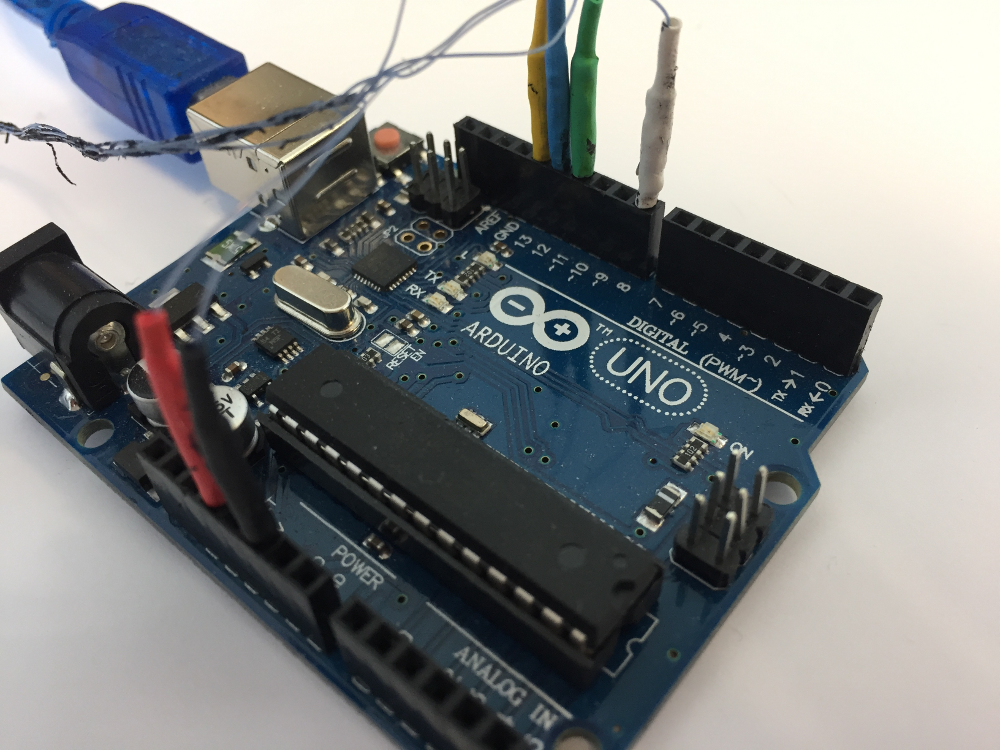
\includegraphics[height=3in]{wiring}
    \end{center}
    \label{fig:wiring}
    \caption{Wiring a single IMU to the Arduino}
\end{figure}



%%%%%%%%%%%%%%%%%%%%%%%%%%%%%%%%%%%%%%%%%%%%%%
%          SECTION: INSTALLATION             %
%%%%%%%%%%%%%%%%%%%%%%%%%%%%%%%%%%%%%%%%%%%%%%

\chapter{Installation}

\section{Arduino IDE}
While there are many ways to install program code onto the Arduino, we have
tested \name{} using the Arduino IDE version 1.8.1. Earlier versions may lack
some of library definitions used by \name{}.

The Arduino IDE can be downloaded from:
\url{https://www.arduino.cc/en/Main/Software}

If your operating system has a package management system, it might be able to
install the Arduino IDE automatically. For example, on a Debian-based system you
can use \texttt{apt}:
\begin{verbatim}
# apt install Arduino-core
\end{verbatim}

\section{Install \name{} on the Arduino}
\label{sec:installarduinocode}

Transfer the file \verb|ic_tx/ic_tx.ino| onto Arduino.  This can be accomplished
using the Arduino IDE graphical user interface.  Alternatively, the Arduino IDE
can be used to program the Arduino directly from the command line:

\begin{verbatim}
# arduino --upload ic_tx/ic_tx.ino
\end{verbatim}

For more information about the Arduino command line interface, see:
\url{https://github.com/arduino/Arduino/blob/master/build/shared/manpage.adoc}


\section{PC}
\label{sec:installPc}

\name{} requires Python 3. It has been tested with Python version 3.5. Thus, it
is recommended to use Python version 3.5 or later. On windows, \name{} has been
successfully installed with the Anaconda Python distribution
(\url{https://www.anaconda.com}), but tests failed to install \name{} with a
standalone Python installation.

It is recommended to use using pip (the Python Package Index) to install
\name{}: \url{https://pypi.python.org/pypi/pip}

\begin{verbatim}
# cd PROGRAM_NAME
# pip install --upgrade pip
# pip install ./
\end{verbatim}

Pip will automatically install any of the following dependencies, and any of their sub-dependencies, if needed:
\begin{itemize}
\item h5py
\item pyqtgraph
\item pyserial
\item pyqt5
\item scipy
\item numpy-quaternion
\end{itemize}

Once \name{} has been installed, it can be started from the command line:\\

\texttt{
\# \name{}
}

On Windows, informational and error messages will not be displayed unless
\name{} is invoked by the Python interpreter explicitly:

\texttt{
\# python \name{}
}

When \name{} starts, the main control panel will be visible (Figure
\ref{fig:control}).

\begin{figure}[]
    \begin{center}
        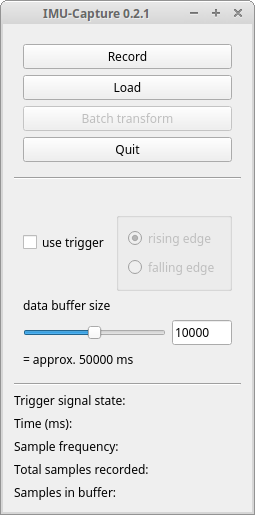
\includegraphics[height=3in]{screenshot_panel}
    \end{center}
    \caption{Control panel} 
    \label{fig:control}
\end{figure}


\chapter{The data buffer} \name{} uses a single data buffer to hold IMU data.
When data is recorded from the IMUs, the data buffer is first erased. Then each
sample is added to the buffer as it is recorded. When data is not being
recorded, the buffer can be saved to a file, or a file can be loaded into the
buffer, erasing any previous contents. Data processing operations can be
performed on the data buffer, altering it irreversibly.  Therefore, any time the
data buffer contains valuable data it is recommended to save it to file before
collecting new data, loading another file, or executing data processing
operations.

The \emph{data buffer length (\# samples)} slider adjusts the size of the data
buffer. When each new sample is received, it is added to the data buffer. If the
buffer is already full (the number of samples in the buffer is equal to the
size of the buffer), the oldest sample in the buffer is deleted. If the size of
the buffer is adjust to be smaller than the number of samples in the buffer, the
oldest samples in the buffer are deleted until the number of samples in the
buffer is equal to the buffer length.


\chapter{Collecting data}

To begin collecting data, press the \emph{record} button.  The \emph{record} button
changes into the \emph{stop} button.  The PC establishes communication with to the
Arduino and instructs it to begin collecting data from the IMUs at 200Hz. This
sample rate is hard-coded, and was determined to be near the maximum possible
with the Arduino Uno.



The \emph{stop} button (or the trigger, as described in Section \ref{sec:trigger}),
causes the PC first to instruct the Arduino to stop collecting data and then to
halt communication with the Arduino.

Table \ref{tab:units} lists the units used for each sensor modality.
\begin{table}
\centering
\begin{tabular}{@{}*3l@{}}
\toprule
instrument & modality & units \\
\midrule 
accelerometer & acceleration          & meters per second squared \\
gyroscope     & rotational speed      & radians per second\\
magnetometer  & magnetic flux density & microteslas \\
\bottomrule
\end{tabular}
\caption{Units used by \name{}}
\label{tab:units}
\end{table}



\section{Plots}
\label{sec:plots}

As samples received from the Arduino are recorded in the data buffer, they
become visible in the data visualization plots. For each IMU, one row of three
plots is displayed. The left-most plot shows accelerometer data, the center plot
shows gyroscope data, and the right-most plot shows magnetometer data. For each
plot, red, green, and blue lines show x, y, and z axis measurements,
respectively.

\begin{figure}[]
    \begin{center}
        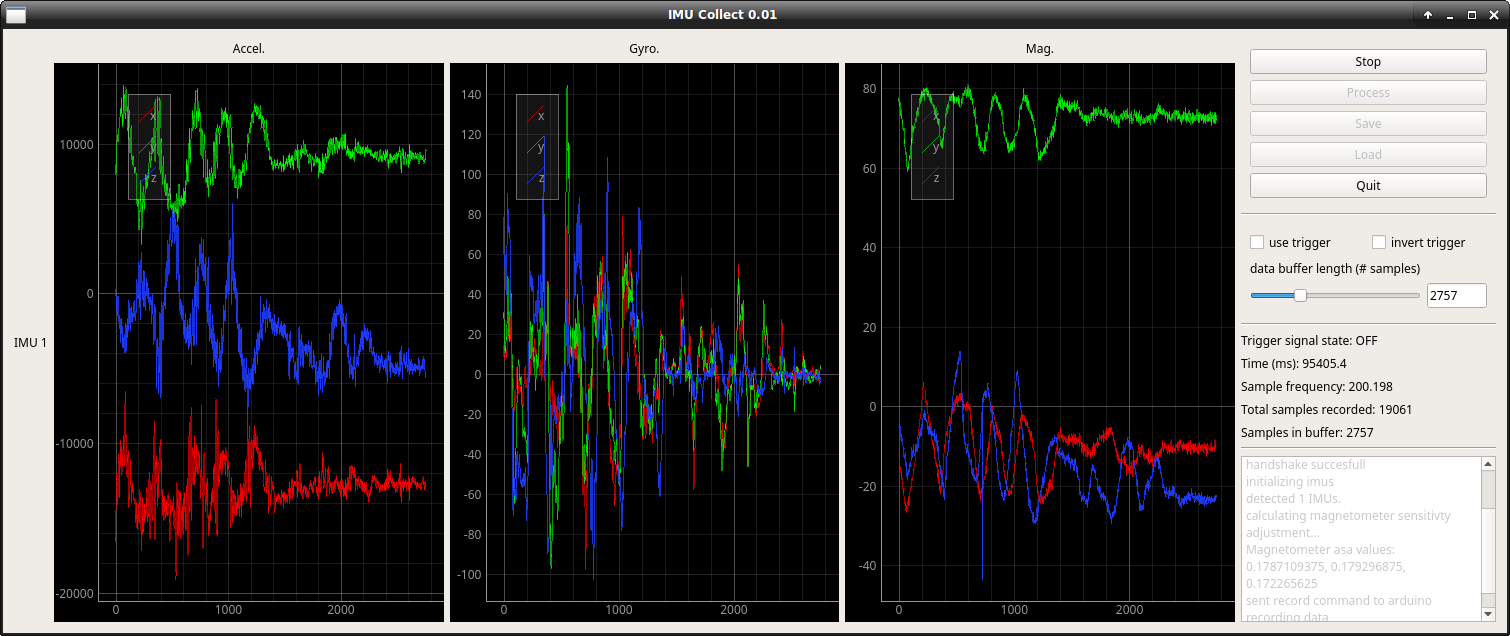
\includegraphics[width=\textwidth]{screenshot_plots}
    \end{center}
    \caption{Collecting data from a single IMU} 
\end{figure}

Each plot will scale automatically as the data buffer is updated. Plots can also
be adjusted manually using the mouse.



\section{Trigger}
\label{sec:trigger}

Optionally, a trigger attached to the Arduino (Section \ref{sec:wiring}) can be
used to stop recording.  If the \emph{use trigger} checkbox is not checked, the
trigger is ignored. Otherwise, if an active trigger is detected, recording will
stop, i.e. the same effect as pressing the \emph{stop} button during recording.
If the \emph{Record} is pressed while the \emph{use trigger} checkbox is checked
and the trigger is active, the recording immediately ends with zero data stored.

If the \emph{invert trigger} checkbox is not checked, the trigger is considered
active when the associated Arduino pin is set high. If the \emph{invert trigger}
checkbox is checked, the trigger is considered active when the associated
Arduino pin is set low.

If no trigger is connected, the value of the pin is undefined.  Thus, to ensure
reliable behavior, the \emph{use trigger} checkbox should be unchecked unless
there is a trigger connected to the Arduino.



\chapter{Saving and loading}
\label{sec:savingloading}

\section{File formats}

\label{sec:fileformats}
The \csv{} file format stores data in plain text, using newlines to delimit
samples and commas to delimit measurements within each sample.  \name{} uses the
CSV module in the Python Standard Library with default formatting parameters:
\url{https://docs.python.org/3/library/csv.html}

The \hdf{} format is designed to store large amounts of data. It is generally
more compact than \csv{}. \name{} uses the h5py Python package to read and write
\hdf{} files: \url{http://www.h5py.org/}


\section{Saving}

The \emph{save} button opens a dialog allowing the user to select a file system
location, a file name, and a file type (either \csv{} or \hdf{}).  The the data
buffer is saved to file according to the selections made in the dialog. The
\emph{save} button is disabled when the data buffer is empty or while data is
being recorded.

\section{Loading}

The \emph{load} button opens a dialog allowing the user to select a file type
(either \csv{} or \hdf{}) and a file to load. The file will be loaded into the
data buffer, overwriting any data stored there.  The \emph{load} button is
disabled while data is being recorded.


\chapter{Filter data}

Due to factors such as the effect of gravity upon the accelerometer, sensor
drift, and noise, the raw data collected by \name{} will not reflect the actual
dynamics of the IMUs. \name{} includes several algorithms that can be applied to
IMU data after it has been recorded. Currently, it is not possible to apply
these algorithms in real time as the data is recorded. Running one of these
algorithms will have to main effects upon recorded data: 1) The effect of
gravity is removed from the acceleration data, leaving only \emph{dynamic}
acceleration. 2) The rotational speed data is converted into rotational angle
data, that is, the rotation of the IMUs is integrated over time.

Currently, filtering algorithms only apply to a single IMU.

The \emph{filter} button opens the data processing control panel (Figure
\ref{fig:filter}).

\begin{figure}[]
    \begin{center}
        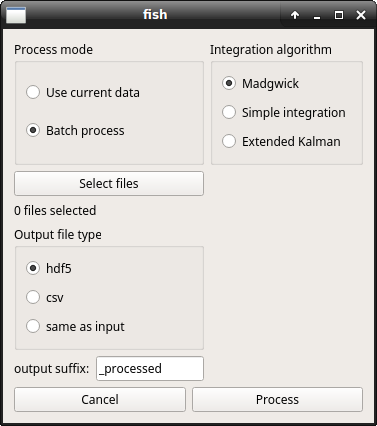
\includegraphics[height=3in]{screenshot_process}
    \end{center}
    \caption{Data filtering control panel} 
    \label{fig:filter}
\end{figure}


\section{Calibration}

Before any of the filtering algorithms can be applied, it is necessary to load a
calibration file by clicking the \emph{Parse calibration file} button. Three
main pieces of information are extracted from the calibration file:
\begin{enumerate}
\item Three orthogonal orientations are used to construct a set of basis vectors
\item The first of the three orientations is used to determine the initial gravity vector
\item The first of the three orientations is used to determine noise covariance matrices
\end{enumerate}


Follow these steps to create a calibration file.

\begin{enumerate}
\item Wire up the IMU as you will use it to collect data
\item Hold the IMU in an orientation to be considered ``upright''
\item Begin recording
\item Hold the IMU upright, in the first orthogonal orientation, for about 5 seconds
\item Rotate the IMU 90 degrees so that the new orientation is orthogonal to the first
\item Hold the IMU in the second orthogonal orientation for about 5 seconds
\item Rotate the IMU 90 degrees again so that the new orientation is orthogonal to both previous orientations
\item Hold the IMU in the third orthogonal orientation for about 5 seconds
\item Stop recording
\end{enumerate}

If \name{} is unable to load a calibration file, error messages explaining why
can help determine if there are problems with the file and help to record a
correct calibration file. See Section \ref{sec:calibErrorMessages} for more
discussion about these messages.


\section{Filter mode}
All data filtering algorithms are applied to the data buffer. If the \emph{Use
current data} radio button is selected, the current contents of the data buffer
are used. This option is not available when the data buffer is empty.

Alternatively, if the \emph{Batch process} radio button is selected, the current
contents of the data buffer are ignored. Instead, batch processing iterates over
a list of one or more input files, loading each file into the data buffer,
applying a filtering algorithm, and saving the result to a new output file
before proceeding to the next input file in the list. The \emph{Select files}
button launches a dialog for selecting input files for batch processing.  The
batch processing output file type can be set, or can vary to match the file type
of each input file. The output suffix string is appended to the file name of each
input file (before the file extension) to compose the output file name. If the
output suffix string is empty and the output file type matches the input
file type, then the input file is overwritten.

With either processing mode, the contents of the data buffer are overwritten by
any data filtering.

\section{Integration algorithm}

The \emph{Integration algorithm} radio buttons select the data filtering
algorithm.

\begin{description}

\item[DSF]
The Dynamic Snap Free algorithm developed by Vikas: (cite)
\item[Madgwick] \hfill
An implementation of the filter developed by Madgwick: 
\url{http://x-io.co.uk/res/doc/madgwick_internal_report.pdf}
\item[Simple integration] \hfill
Use the Madgwick algorithm with the beta parameter set to 0.

\end{description}





\chapter{Troubleshooting}

\section{Installation}

If you encounter problems during installation, make sure you are using Python
3.5 or later and that pip is working with the correct Python version.


\section{General error messages}

This sections discusses some of the error messages that may be reported by
\name{}.


\newcommand{\genericFix}{Try resetting the Arduino.  Make sure that the Arduino
is correctly powered and connected to the PC (Section \ref{sec:wiring}), and
that the correct code is installed on the Arduino (Section
\ref{sec:installarduinocode}).}

This section provides explanation and troubleshooting tips for each error
message produced by \name{}.

\begin{description}

\item[ASA read failed, using 1 adjustment]
For each magnetometer axis, a sensitivity adjustment value (ASA) is stored in
ROM by the manufacturer.  This error message is reported when the Arduino is
unable to read the ASA values from an IMU.  It likely indicates that the Arduino
is not communicating correctly with the magnetometer.  Any magnetometer data
recorded after this message should be discarded.
\genericFix{}

\item[failed to create connection, aborting]
The program failed to establish a serial connection with the Arduino.
\genericFix{}

\item[handshake failed]
Even though the PC may have established a valid serial connection to the
Arduino, the data exchange protocol used by \name{} failed to establish a
communication handshake with the Arduino.
\genericFix{}
It is possible the \name{} incorrectly identified a serial device as the
Arduino. Any device that the pySerial library
(\url{https://pythonhosted.org/pyserial/#}) identifies as manufactured either by
``Arduino'' or by ``Microsoft'' will be identified as an Arduino by \name{}. Try
disconnecting all serial devices and then reconnecting them, starting with the
Arduino.

\item[invalid csv file]
The program attempted to read a .csv file (Section \ref{sec:fileformats}), but
the format of the data in the file was not valid.

\item[invalid file type:\ldots]
There was an attempt either to save or to load a file type other than
\csv{} and \hdf{}. As discussed in Section \ref{sec:fileformats},
\csv{} and \hdf{} are the only file formats supported by \name.

\item[no Arduino found]
The program searched for Arduinos on all serial ports but didn't find any.
\name{} uses the pySerial library to scan for Arduinos:
\url{https://pythonhosted.org/pyserial/#}

\item[no IMUs detected, aborting]
The Arduino did not detect any attached IMUs.  After the Arduino is initialized,
it attempts to determine the number of IMUs by sending a WHOAMI request while
signaling each of the three legal chip select pins (Section \ref{sec:wiring}).
It then sends a message to the PC reporting the number of responses received. This
error is reported if the Arduino does not receive any WHOAMI responses.
\genericFix{}

\item[rx failed, no data read from serial]
The PC expected to receive data from the Arduino but failed. Perhaps no data was
transmitted, or perhaps data that violates the communication protocols used by
\name{} was received.
\genericFix{}

\item[unknown sample received:\dots]
The PC expected to receive a packet containing a data sample, but the packet
either had the wrong type or the wrong length. This message can be ignored if it
occurs only briefly at the beginning of recording. Otherwise, try resetting the
Arduino.

\item[unable to determine number of IMUs, aborting]
The program failed to determine how many IMUs are attached to the Arduino. After
the Arduino is initialized, it attempts to determine the number of IMUs by
sending a WHOAMI request while signaling each of the three legal chip select
lines (Section \ref{sec:wiring}). It then sends a message to the PC reporting the
number of IMUs detected. This error is reported if the PC sends a
command to the Arduino to initialize, but does not receive a message reporting
the number of IMUs detected.
\genericFix{}

\end{description}

\section{Calibration error messages}
\label{sec:calibErrorMessages}

This section discusses error messages that may be reported when \name{} fails
to load a calibration file.

\begin{description}

\item[fewer than 3 steady intervals]
A ``steady interval'' is a contiguous duration of at least 3 seconds when the
change in accelerometer measurement remains below a threshold and and the
gyroscope measurement remains below a threshold. Possibly the IMU was not held
still enough, or the duration of one or more hold was too short.

\item[too many steady intervals, the limit is\ldots]
See the discussion for ``fewer than 3 steady intervals'' for a definition of
``steady interval''.  \name{} can remove some some extra steady intervals if
they are not part of a triple of orthogonal vectors, but too many will cause
this error. When recording the calibration file, start recording when with the
IMU in the first orientation, end recording immediately after 5 seconds of the
third orientation, and make smooth, quick, transitions between the orientations.

\item[found more than 1 triple of orthogonal vectors]
More than three orientations were recorded, and more than one triple of
orthogonal vectors can be identified.  This is similar to ``too many steady
intervals, the limit is\ldots''. See the discussion of that message for possible
solutions.

\item[could not find 3 orthogonal vectors]
Even though at least 3 ``steady intervals'' (see the discussion of the ``fewer
than 3 steady intervals'' message) were found, no 3 intervals are orthogonal.
That is, the difference between 90 degrees and the angles separating the
intervals was greater than a threshold. When recording the calibration file,
ensure that that three orientations are mutually orthogonal.


\end{description}

\end{document}
